\chapter{Evaluation}
\label{sec:evaluation}


% Zu jeder Arbeit in unserem Bereich gehört eine Leistungsbewertung. Aus
% diesem Kapitel sollte hervorgehen, welche Methoden angewandt worden,
% die Leistungsfähigkeit zu bewerten und welche Ergabnisse dabei erzielt
% wurden. Wichtig ist es, dem Leser nicht nur ein paar Zahlen
% hinzustellen, sondern auch eine Diskussion der Ergebnisse
% vorzunehmen. Es wird empfohlen zunächst die eigenen Erwartungen
% bezüglich der Ergebnisse zu erläutern und anschließend eventuell
% festgestellte Abweichungen zu erklären.

Es wurden nun unterschiedliche Verschlüsselungsalgorithmen vorgestellt und in das aktuelle \gls{MACsec Modul} implementiert.
Im Folgenden werden Performance Tests durchgeführt, um zu sehen, ob dadurch eine höhere Datenübertragungsrate und niedrigere Latenz erreicht werden kann.\\
Leider war es nicht möglich, MORUS640 und AEGIS128L mit dem software-optimierten Implementationen zu testen. Die Implementationen werden erst ab dem Linux Kernel 4.18 unterstützt, der zum Zeitpunkt der Test noch nicht funktionsfähig zur Verfügung stand. Deshalb mussten die Implementationen zu einer älteren Kernel-Version hinzugefügt werden, wodurch noch keine Softwareoptimierungen unterstützt werden können. In \ref{sec:software benchmarking} wurde gezeigt, wie sehr sich die Optimierungen auf die Performance auswirken. Daher ist zu erwarten, dass die fehlenden Optimierungen negative Auswirkungen auf die Latenz und Datenübertragungsrate von MORUS640 und AEGIS128L haben.
\section{Testaufbau}\\
\\
Die Testergebnisse werden auf zwei Rechnern evaluiert, die mittels eines LAN-Kabels miteinander verbunden sind.
Auf den Rechnern läuft folgende Hardware:
\begin{table}[hp]
\centering
\begin{tabular}{cccc}
\multicolumn{2}{l}{Prozessor:} \multicolumn{2}{r}{Intel i5-4590 3.3GHz} \\ 
\multicolumn{2}{l}{RAM:} \multicolumn{2}{r}{16GB}\\ 
\multicolumn{2}{l}{Betriebssystem:} \multicolumn{2}{r}{Ubuntu 18.04 mit dem Linux-Kernel 4.15.0-32} \\ 
\end{tabular} 
\caption[Testaufbau]{In der Tabelle wird die Hardware des Systems aufgelistet.}
\end{table}\\Jeder Algorithmus wird mit verschiedenen Paketgrößen getestet, um reale Bedingungen zu simulieren.
Dabei wird geschaut, ob die unterschiedlichen Paketgrößen Auswirkungen auf die Latenz oder die Datenübertragungsrate haben. Die Datenübertragungsrate kann mit dem Werkzeug iperf3 gemessen werden. Neben der Bandbreite sind die Latenz und die CPU Auslastung entscheidende Messkriterien. Dafür bietet sich das Werkzeug ping an. Damit lässt sich die Round-trip time feststellen. Das ist die zeitliche Übertragung eines festen Pakets zum Zielrechner und die Beantwortung des Pakets vom Zielrechner.
Folgende Tests werden durchgeführt:
\begin{enumerate}
\item \gls{MACsec} wird mit den Verschlüsselungsalgorithmen \gls{AES-GCM}, ChaCha20-Poly1305 , AEGIS128L und MORUS640 mit ping getestet. Die verwendeten Paketgrößen sind 128, 256, 512, 1024, 1400 und 1514 Bytes. Die Tests werden sowohl mit Verschlüsselung als auch ohne Verschlüsselung ausgeführt.
\item MACsec wird mit den Verschlüsselungsalgorithmen AES-GCM, ChaCha20-Poly1305 , AEGIS128L und MORUS640 mit iperf3 getestet. Die verwendeten Paketgrößen sind 128, 256, 512, 1024, 1400 und 1514 Bytes. Die Tests werden sowohl mit Verschlüsselung als auch ohne Verschlüsselung ausgeführt.
\item Ethernet wird mit den Paketgrößen 128, 256, 512, 1024, 1400 und 1514 Bytes mit iperf3 und ping getestet.
\end{enumerate}
Die verwendeten Paketgrößen sind gängige Größen, um Verschlüsselungsalgorithmen zu testen. Daher werden diese Werte übernommen, um leichter Vergleiche zu anderen Arbeiten ziehen zu können.
Die Auswertungen werden mit einem Bash-Skript ausgeführt, welches auf beiden Testrechnern die Konfigurationen mit den unterschiedlichen Paketgrößen und Verschlüsselungsalgorithmen via \gls{SSH} aktualisiert und die Analyse mit ping oder iperf3 startet.
Iperf3 sendet in einem Zeitraum von 10 Sekunden Pakete an einen Server, der auf dem Empfängerrechner konfiguriert wurde und misst jede Sekunde den durchschnittlichen Datendurchsatz. Die Resultate der Testsoftware werden in eine Datei geschrieben und gespeichert. In eine Datei wird jeweils nur ein Test mit einem Verschlüsselungsalgorithmus und nur einer Paketgröße geschrieben. Im Zuge der Datenanalyse hat sich herausgestellt, dass die Daten leichter zu untersuchen sind, wenn sie sich in einer Datei befinden. Daher wurden im Nachhinein alle Dateien eines Verschlüsselungsalgorithmus mit unterschiedlichen Paketgrößen konkateniert und zu einer Datei gebündelt, was zu einer Erleichterung der Datenanalyse führte.\\
Die iperf3 Tests wurden mit \gls{AES-GCM} und ChaCha20-Poly1305 für jede Paketgröße 250 mal wiederholt. Die Evaluation von MORUS640 und AEGIS128L konnten aufgrund von Implementationsproblemen erst später durchgeführt werden und wurden aus Zeitgründen 100 mal für jede Paketgröße wiederholt. \\
Die ping Tests wurden 50000 mal für jede Paketgröße wiederholt. Normalerweise wird eine ping Anfrage in einem festen Intervall gesendet, der eine Sekunde beträgt. Mit der adaptiven ping Option kann der Testvorgang beschleunigt werden, indem die ping Anfragen sofort gesendet werden, sobald die vorherige Anfrage beantwortet wurde. 
\subsection{Datendurchsatz}
\\
\\
In Abbildung \ref{img:bytes-e} und \ref{img:bytes-we} sind die Ergebnisse der Evaluation in Diagrammen dargestellt.
Aus den Diagrammen ist ersichtlich, dass es keinen Unterschied macht, ob \gls{MACsec} die Daten verschlüsselt und dann den TAG bildet oder die Verschlüsselung auslässt und nur den TAG generiert. Das ist damit zu erklären, dass bei \gls{AEAD} Algorithmen die Verschlüsselung und Tag Bildung in der gleichen Verschlüsselungsrunde durchgeführt werden. Deshalb benötigt ein Algorithmus trotzdem die gleiche Anzahl an Zyklen, um einen TAG zu einer Nachricht zu bilden,
egal ob Verschlüsselung angewendet wird oder nicht. Des Weiteren sieht man, dass noch Verbesserungspotenzial im Vergleich zur Ethernet möglich ist, wenn ein Verschlüsselungsalgorithmus mit einer niedrigen Paketgröße ausgewählt wurde. Allerdings kann jeder Algorithmus die Leitung komplett auslasten, sobald eine Paketlänge von 1024 Bytes erreicht wird. \gls{AES-GCM} und ChaCha20-Poly1305 haben sehr ähnliche Testergebnisse. ChaCha20-Poly1305 kann also von der Performance durchaus eine Alternative zu \gls{AES-GCM} sein. MORUS640 und AEGIS128L schließen ab einer Paketlänge von 1024 Bytes mit ChaCha20-Poly1305 und AES-GCM auf. Bei niedrigen Paketlängen erreicht MORUS640 knapp die Hälfte des Durchsatzes von AES-GCM. AEGIS128L ist im Vergleich zu MORUS640 ein wenig schneller und kann bereits ab einer Paketlänge von 512 Bytes zu \gls{AES-GCM} und ChaCha20-Poly1305 aufholen. Die genauen Testresultate findet man in der Appendix in den Tabellen \ref{tab:bytes-e} und \ref{tab:bytes-we} .
\afterpage{%
\begin{figure}[!p]
\centering
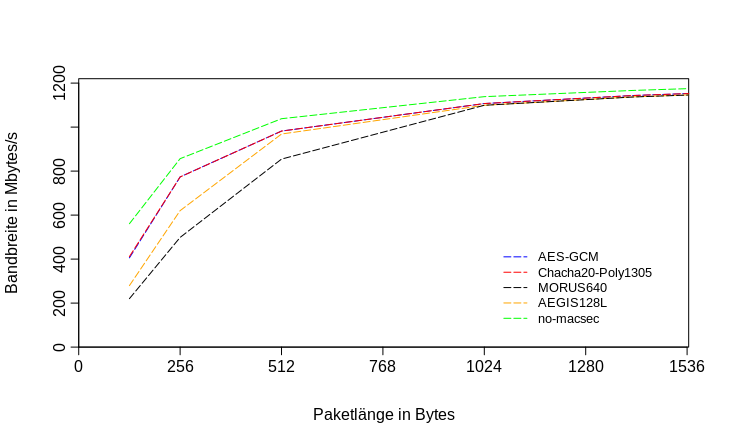
\includegraphics[width=0.95\textwidth]{images/bytese-new.png}
\caption[Bandbreite Diagramm mit aktivierter Verschlüsselung]{In dem Diagramm wird die Bandbreite der Verschlüsselungsalgorithmen in mbytes/s dargestellt. Die Test wurden mit aktivierter Verschlüsselung durchgeführt.}
\label{img:bytes-e}
\end{figure}
\begin{figure}[!p]
\centering
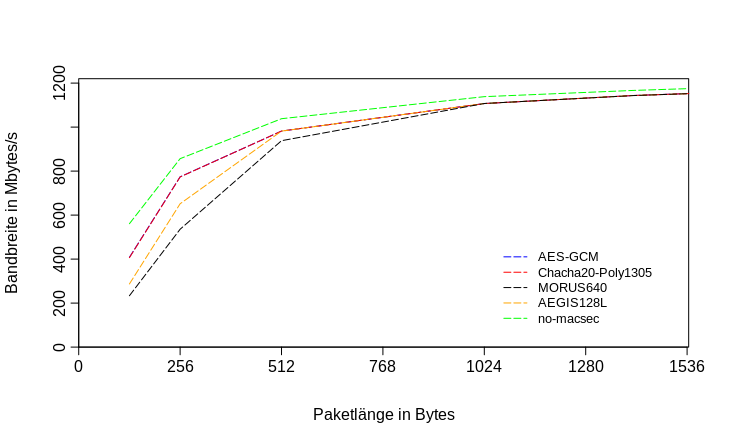
\includegraphics[width=0.95\textwidth]{images/bytes-we-new.png}
\caption[Diagramm der Bandbreite ohne Verschlüsselung]{In dem Diagramm wird die Bandbreite der Verschlüsselungsalgorithmen in mbytes/s dargestellt. Die Test wurden ohne Verschlüsselung durchgeführt.  }
\label{img:bytes-we}
\end{figure}
\clearpage
}
\subsection{CPU Auslastung}
\\
\\
Während der iperf3 Testvorgänge wurde gleichzeitig die CPU Auslastung des Computers ermittelt. Die Testergebnisse sind in den Diagrammen \ref{img:CPU-E} und \ref{img:CPU-WE} aufzufinden. Zusätzlich gibt es in der Appendix in den Tabellen \ref{tab:CPU-e} und \ref{tab:CPU-we} die genauen Resultate. Die Daten zeigen, dass alle hinzugefügten Algorithmen eine hohe \gls{CPU} Auslastung bei niedrigen Paketgrößen aufweisen. Bei MORUS640 ist ein sogenannter Bottleneck bei den Paketgrößen erkennbar. Das heißt, dass MORUS640 die CPU komplett auslastet und somit die Performance von MORUS640 durch die CPU gedrosselt wird. Die \gls{CPU} Auslastung bei MORUS640 liegt bei den Paketgrößen 128, 256 und 512 Bytes im Schnitt bei 96,8 Prozent. Die enorme Belastung der CPU in den niedrigen Paketgrößen lässt sich dadurch erklären, dass bei geringen Paketgrößen die Verschlüsselungsalgorithmen wesentlich häufiger aufgerufen werden müssen als bei großen Paketgrößen. Der häufige Funktionsaufruf führt auch bei ChaCha20-Poly1305 zu einer hohen CPU Auslastung. Diese liegt im Durchschnitt bei 96,6 Prozent, wenn eine Paketlänge von 128 benutzt wird. Einzig und allein \gls{AES-GCM} hat durchgängig eine durchschnittliche CPU Auslastung von knapp einem Prozent und liegt damit fortwährend sehr nah an der CPU Auslastung von Ethernet und erzielt in einigen Fällen sogar bessere Ergebnisse als die Ethernet. Dies lässt sich nur durch Messungenauigkeiten in den Resultaten erklären.
\subsection{Latenz}
\\
\\
Die Paketumlaufzeit ist in der Appendix in den Tabellen \ref{tab:Lat-e} und \ref{tab:Lat-we} aufzufinden.
Auch bei der Latenz weist \gls{AES-GCM} die besten Resultate auf mit einer durchschnittlichen Zeit von 0,143 ms bei einer Paketgröße von 128 Bytes und 0,147 ms bei 1514 Bytes. Die Latenz ist nur minimal größer als die von Ethernet mit 0,136 ms bei 128 Bytes und ist in einigen Fällen sogar etwas besser mit 0,15 bei 1514 Bytes. Das ist erneut durch eine Messungenauigkeit erklärbar. MORUS640 und AEGIS128L haben mit Abstand die höchste Latenz, die im Schnitt bei 0,162 ms bei AEGIS128L und 0,16 ms bei MORUS640 liegt. AEGIS128L ist somit 10 Prozent langsamer als \gls{AES-GCM} mit einer durchschnittlichen Zeit von 0,145 ms. Ein Grund dafür könnte die fehlende Software Optimierung sein. Daher wurden diese Ergebnisse, wie bereits in der Einleitung des Kapitels erwähnt, erwartet. Auffallend ist die geringe Varianz von ChaCha20-Poly1305 und AES-GCM. Die durchschnittliche Paketumlaufzeit zwischen den Paketlängen hat bei ChaCha20-Poly1305 nur eine Differenz von 0,005 ms und ist nur noch bei AES-GCM minimal geringer mit 0,004  ms. Daraus lässt sich eine konstante Performance von AES-GCM und ChaCha20-Poly1305 erkennen. Die Diagramme sind in der Appendix \ref{img:AEGISping} aufzufinden.
\afterpage{%
\begin{figure}[!p]
\centering
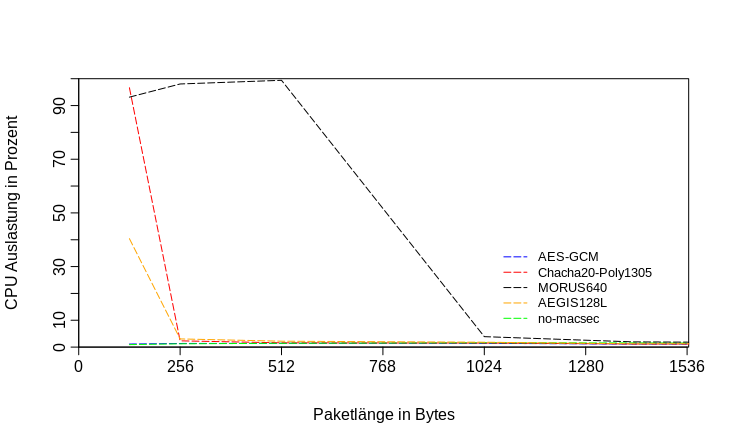
\includegraphics[width=0.95\textwidth]{images/CPU-E-NEW.png}
\caption[CPU Auslastung mit aktivierter Verschlüsselung]{Das Diagramm zeigt die CPU Auslastung in Prozent der einzelnen Verschlüsselungsalgorithmen, Während der Tests wurde die Verschlüsselung aktiviert.  }
\label{img:CPU-E}
\end{figure}
\begin{figure}[!p]
\centering
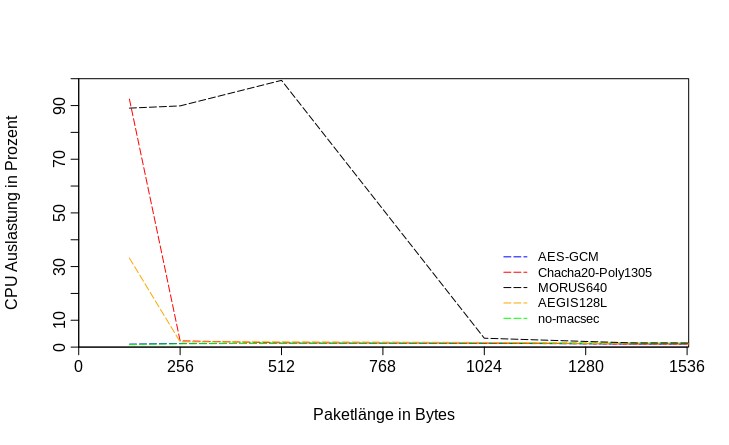
\includegraphics[width=0.95\textwidth]{images/cpu-we-new.png}
\caption[CPU Auslastung ohne Verschlüsselung]{Das Diagramm zeigt die CPU Auslastung in Prozent der einzelnen Verschlüsselungsalgorithmen, Während der Tests wurde keine Verschlüsselung verwendet. }
\label{img:CPU-WE}
\end{figure}
\clearpage
}
\section{Sicherheitsevaluation}
\label{sec:sicherheitsevalutation}
\\
\\
Der Sicherheitsstandard MACsec garantiert folgende Sicherheitsziele: Vertraulichkeit, Integrität, Authentizität, bounded receive delays und Schutz vor Replay Angriffen. Im folgenden Abschnitt wird auf die Änderungen eingegangen, die in Kapitel \ref{sec:implementation} beschrieben worden sind und ob diese Auswirkungen auf die genannten Sicherheitsmerkmale haben. Im Rahmen der Bachelorarbeit wird es nicht möglich sein, komplette Sicherheitsanalysen der einzelnen Algorithmen vorzustellen, daher werden nur die wichtigsten Kriterien behandelt. Im kompletten Abschnitt wird davon ausgegangen, dass die Algorithmen korrekt verwendet werden.
\subsection{Vertraulichkeit}
Da ein Verschlüsselungsalgorithmus maßgeblich für das Sicherheitsziel der Vertraulichkeit verantwortlich ist, muss man sehr sorgfältig überprüfen, ob die gemachten Änderungen einen Einfluss auf die Sicherheit haben.
Es wurden insgesamt 3 weitere Verschlüsselungsalgorithmen implementiert. \\
\\
\textbf{ChaCha20-Poly1305}
\\
\\
ChaCha20-Poly1305 besitzt eine Schlüssellänge von 256-Bits und ist somit doppelt so lang wie die Schlüssellänge von \gls{AES-GCM}. Desweiteren bietet ChaCha20-Poly1305 wenig Angriffsfläche gegenüber "timing-attacks", die bei \gls{AES-GCM} gefunden wurden\cite{cache-collision-timing-attacks-against-aes}. Somit kann sogar eine höhere Sicherheit der Vertraulichkeit gewährleistet werden als bei AES-GCM. An dieser Stelle muss erwähnt werden, dass die Implementation von ChaCha20-Poly1305 nur mit einem statischen Schlüssel erfolgen konnte. In diesem Fall wirkt sich der geringe Initialisierungsvektor negativ aus, da mit einem Initialisierungsvektor der Länge von 96-Bit nur ca 256 Gigabyte verschlüsselt werden können, ohne das sich der Initialisierungsvektor wiederholt\cite{rfc7539}. In Anbetracht der Tatsache, dass die Implementierung des Autors von ChaCha20-Poly1305 nur einen Prototyp darstellt, um Performance-Analysen ausführen zu können, ist die Schwächung der Sicherheit von \gls{MACsec} durch einen statischen Schlüssel vernachlässigbar, da eine korrekte Implementierung von ChaCha20-Poly1305 die Sicherheit des MACsec Moduls nicht beeinträchtigen würde.\\
\\
\textbf{AEGIS128L, MORUS640}
\\
\\
AEGIS128L und MORUS640 benutzen jeweils eine Schlüssellänge von 128-Bits. In der wissenschaftlichen Publikation von AEGIS128L\cite{10.1007/978-3-662-43414-7_10} und MORUS640\cite{wuauthenticated} ist eine genaue Sicherheitsanalyse zu den Algorithmen zu finden. Allerdings existiert noch kein formaler Sicherheitsbeweis für die beiden Algorithmen. Dies könnte daran liegen, dass die Algorithmen erst 2014 publiziert worden sind. Aus diesem Grund können AEGIS128L und MORUS640 noch nicht zu den wohluntersuchten Algorithmen gezählt werden. Das hat keine negativen Auswirkungen auf das Sicherheitsziel der Vertraulichkeit, aber bei der Anwendung von AEGIS128L und MORUS640. Dementsprechend sollte bei der Anwendung von AEGIS128L und MORUS640 weniger Vertrauen entgegengebracht werden.

\subsection{Integrität}
\\
\\
Da der Betriebsmodus \gls{AEAD} verwendet wird, wird auch Message Authentication Code ausgetauscht, sobald eine andere Chiffre verwendet wird. Deshalb muss der verwendete Message Authentication Code der einzelnen Chiffren betrachtet werden. Der Aufbau der Message Authentication Codes wurde bereits in \ref{sec:aegis} und \ref{sec:chacha20-poly1305} genauer erläutert. \\
\\
\textbf{Poly1305}
Die Nutzung von Poly1305 hat keinen negativen Effekt auf die Integrität des Sicherheitsstandards.
\\
\\
\textbf{AEGIS128L, MORUS640}
\\
\\
Trotz eines fehlenden Sicherheitsbeweises wird in \cite{10.1007/978-3-662-43414-7_10} und \cite{wuauthenticated} explizit hervorgehoben, dass AEGIS128L und MORUS640 eine 128-Bit Sicherheit für Authentikation bereitstellen können, die höher ist als die von \gls{AES-GCM}. Demzufolge wird die Sicherheit der Integrität bei der Anwendung von MORUS640 und AEGIS128L verstärkt.\\
\\
\textbf{Authentizität}
\\
\\
Da die Authentizität durch den ICV des MACsec Standards gesichert und der \gls{ICV} durch den Message Authentication Code gebildet wird, schwächt dies nicht die Authentizität, weil in diesem Abschnitt gezeigt wurde, dass ein Austausch des Verschlüsselungsalgorithmus keine negativen Auswirkungen auf die Integrität ausübt.
\subsection{Verfügbarkeit}
\\
\\
Im Sicherheitsstandard wurden nur zusätzliche Verschlüsselungsalgorithmen hinzugefügt. Diese Änderungen können Auswirkungen auf die Vertraulichkeit oder Integrität haben. Allerdings hat ein anderer Verschlüsselungsalgorithmus keinen Effekt auf die Verfügbarkeit, solange das \gls{MACsec} Modul korrekt verwendet wird und kein aktiver Angriff auf das System vorliegt. Darüber hinaus hat ein aktiver Angriff keine Auswirkungen auf die Funktionsweise des Verschlüsselungsalgorithmus.
\subsection{Replay Angriffe}
\\
\\
\gls{MACsec} schützt vor Replay Angriffen, in dem jedes versendete Paket eine Paketnummer zugeteilt bekommt, die nach jedem Paket inkrementiert wird. Wiederholt sich eine Paketnummer, so wird das Paket abgelehnt. Zwar wurden aufgrund der Paketnummer Änderungen am SecTag vorgenommen, das beschränkt sich allerdings nur auf die Vergrößerung des Paketnummer Feldes, um größere Initialisierungsvektoren zu unterstützen. Trotzdem wird der vergrößerte SecTag weiterhin komplett vom \gls{ICV} geschützt, sodass keine neuen Angriffsmöglichkeiten auf den SecTag bestehen.\clearpage
\section{Resultate}
Die Ergebnisse fallen durchmischt aus. 
ChaCha20-Poly1305 kann größtenteils bei der Bandbreite und \gls{CPU} Auslastung mit \gls{AES-GCM} mithalten. Auch bei der Latenz ist ChaCha20-Poly1305 im Schnitt nur 4,1 Prozent langsamer als \gls{AES-GCM}, was ein tolerierbarer Wert ist. Anders sehen die Ergebnisse bei AEGIS128L und MORUS640 aus. Die Daten zeigen, dass die Latenz von MORUS640 und AEGIS128L weit hinter denen von ChaCha20-Poly1305 und \gls{AES-GCM} liegen. Wenn die Bandbreite betrachtet wird, können AEGIS128L und MORUS640 bei geringen Paketgrößen auch nicht mithalten. Trotzdem muss erwähnt werden, dass Software Optimierungen große Auswirkungen auf einen Algorithmus haben können\cite{Ankele2016SoftwareBO} und sowohl AEGIS128L als auch MORUS640 zum Zeitpunkt der Experimente keinen Zugriff auf deren Optimierungen hatten. In Anbetracht dieser Tatsache fallen die Ergebnisse von MORUS640 und AEGIS128L durchaus akzeptabel aus. Insgesamt zeigt sich, dass auf dieser Testumgebung die aktuelle ChaCha20-Poly1305 Implementation durchaus eine ernsthafte Alternative zu \gls{AES-GCM} bieten kann.


%%% Local Variables:
%%% TeX-master: "diplom"
%%% End:
